\documentclass[a4paper,12pt]{article}   % 文檔類型為article
\usepackage{setspace}
\usepackage{fontspec}% 使用系统字体
\usepackage{xeCJK}    % 提供中文支持

% 设置中文正文字体为標楷體,你需要确保系统上有標楷體字体文件
\setCJKmainfont{標楷體}

%\onehalfspacing % 1.5 倍行距,與 Word 中的默認行距相同
%\pagestyle{empty}

\setmainfont{Times New Roman}
\fontsize{12pt}{\baselineskip}   % 設置字體大小為12pt,行距為單行


\usepackage{pdfpages}
\usepackage{enumitem}
\usepackage{fontspec}
\usepackage{authblk} 
\usepackage{titlesec}
\usepackage{amssymb}
\usepackage{graphicx}
\usepackage{titlesec}
\titlespacing{\section}{0pt}{*2}{*1}
\titlespacing{\subsection}{0pt}{*2}{*1}
\titlespacing{\subsubsection}{0pt}{*2}{*1}

\usepackage{tabularx}
\usepackage{multirow}
%\usepackage{colortbl}
\usepackage{amsthm}
\usepackage{booktabs} % 用於漂亮的表格樣式


\usepackage{colortbl} % 用於表格顏色
\usepackage{xcolor}   % 用於文本顏色
\definecolor{lightgray}{gray}{0.9} % 自定義顏色

\pagestyle{plain}


\begin{document}
%\maketitle

\begin{center}
	{\fontsize{16pt}{12pt}\selectfont Self-supervised and transfer learning on CIFAR10}
	
\end{center}

\hfill  B092040016 陳昱逢
	
	
\begin{center}
	Assignment 4
\end{center}

\section{Task 1}
	在旋轉預測任務中訓練隨機初始化權重的 ResNet18,我在訓練完後對測試集的旋轉預測的準確率達到 \textbf{78.99\%},經過多次實驗,訓練完後的準確率大約落在 78 - 80\% 之間,我採用的優化器是 AdamW, Table\ \ref{table:param} 呈現了我此次實驗的參數。 論文\ \cite{gidaris2018unsupervised} 提出先預測旋轉的任務作為無監督學習再應用到其他視覺任務時會有不錯的效果, 我認為這個任務有這樣的泛化性可能原因是如果模型可以成功預測出他旋轉了幾度、旋轉的類別,那麼這個模型其實已經有學到了一些關於圖片裡的一些語義或資訊,因此才可以再應用到其他下游任務中進行 fine-tune,且效果比起重新訓練隨意初始化的模型還要好。
	
	
\begin{table}[htb]
	\centering	
	\normalsize
    \newcommand{\z}{\phantom{0}}
    \caption{configurations of my experiment}
    \vspace{0.15\baselineskip}
    \resizebox{0.6\textwidth}{!}{
		\begin{tabular}[c]{|l|l|}
			\hline
			\textbf{parameter} & \textbf{configuration} \\
			\hline
			num\_epochs   &  45 \\
			\hline
			decay\_epochs & 15 \\
			\hline
			init\_lr & 0.01  \\
			\hline
			AdamW & weight\_decay = 0.01 \\
    			\hline
		\end{tabular}
	}
	\label{table:param}
   \vspace{0.1\baselineskip}
\end{table}



\section{Task2}

	此任務將採用前面訓練好的 rotation model (RotNet) 或是隨機初始化權重的模型, fine-tune 最後一層的卷積層 (convolution layer) 以及全連接層 (fully connected layer; FC) 在利用 CIFAR10 資料集進行監督式學習的分類任務。


\subsection{採用訓練在旋轉預測的 RotNet 模型}
	此部分採用預訓練好的 RotNet 模型並 fine-tune 最後一層卷積層以及 FC 層,我在訓練後對 CIFAR10 測試集分類任務的準確率達到 \textbf{62.09\%},相比隨機初始化權重的模型提高了 16.78\%,可見預訓練的旋轉預測任務有理解圖片中的一些語義或資訊。此實驗的參數 num\_epochs 設為 20, decay\_epoch 設為 10, init\_lr 同樣設為 0.01。經過實驗多次後,有趣的是我發現此任務的準確率很跳動,即便在我預訓練模型的準確度都很相似的情況下,我有些時候此任務的分類任務最後準確率只有大約達到 57\%,每次實驗結果都會有些誤差,我猜測可能原因是初始的點挑的不好,導致在找 loss 最低點的時候提前遇到了梯度較小的地方,很難找到最佳值。

	
\subsection{採用隨機初始化權重的模型}
	此部分採用隨機初始權重的 ResNet18 並 fine-tune 最後一層卷積層以及 FC 層,我在訓練後對 CIFAR10 測試集分類任務的準確率達到 45.31\%。此實驗的參數同樣將 num\_epochs 設為 20, decay\_epoch 設為 10, init\_lr 設為 0.01。 Table\ \ref{table:comparison1} 呈現了兩個模型的準確度比較,可以觀察到經過預訓練的 RotNet 模型相比隨機初始化權重的 ResNet18 模型提高了 16.78\%,可見經過預訓練的旋轉預測任務可以有效的應用到其他視覺任務中,也驗證了旋轉預測有助於理解圖片中的一些語義或資訊。
	
	
\begin{table}[htb]
	\centering	
	\normalsize
    \newcommand{\z}{\phantom{0}}
    \caption{Simulation results of each model}
    \vspace{0.15\baselineskip}
    %\resizebox{0.5\textwidth}{!}{
	\begin{tabularx}{0.6\textwidth}{@{}lr@{}}\toprule
		\textbf{Model} & \textbf{Accuracy} \\
		\hline
		pre-trained RotNet model & \textbf{0.6209}  \\ 
		random initialized ResNet18   & 0.4531  \\
    		\hline

	\end{tabularx}
	%}
	\label{table:comparison1}
   \vspace{0.15\baselineskip}
\end{table}


\section{Task 3}
	
	此任務與任務二相似,將採用前面訓練好的 rotation model (RotNet) 或是隨機初始化權重的模型來對 CIFAR10 做圖片分類, 不過在訓練時可以調整整個模型的架構。
	
\subsection{採用訓練在旋轉預測的 RotNet 模型}
	此部分採用預訓練好的 RotNet 模型並調整整個網路架構,我在訓練後對 CIFAR10 測試集分類任務的準確率達到 \textbf{84.11\%},相比重新訓練隨機初始化權重的模型提高了 1.78\%,此實驗的參數同樣將 num\_epochs 設為 20, decay\_epoch 設為 10, init\_lr 設為 0.01。


\subsection{採用隨機初始化權重的模型}
	此部分的實驗採用隨機初始化權重的 ResNet18 重新訓練,我在訓練後對 CIFAR10 測試集分類任務的準確率達到 82.33\%。此實驗的參數同樣將 num\_epochs 設為 20, decay\_epoch 設為 10, init\_lr 設為 0.01。 Table\ \ref{table:comparison2} 呈現了兩個模型的準確度比較,可以觀察到經過預訓練的 RotNet 模型相比隨機初始化權重的 ResNet18 模型提高了 1.78\%,雖然提升的沒有很明顯,但我發現在第一輪 epoch 時,經過預訓練的 RotNet 模型在測試集的分類表現就已經達到 64.69\% 的準確度,而隨機初始權重在第一輪 epoch 時僅有 40.66\% 的準確率。由此可見,旋轉預測真的可以幫助模型學到圖片裡的一些資訊。 


\begin{table}[htb]
	\centering	
	\normalsize
    \newcommand{\z}{\phantom{0}}
    \caption{Simulation results of each model}
    \vspace{0.15\baselineskip}
    %\resizebox{0.5\textwidth}{!}{
	\begin{tabularx}{0.6\textwidth}{@{}lr@{}}\toprule
		\textbf{Model} & \textbf{Accuracy} \\
		\hline
		pre-trained RotNet model & \textbf{0.8411}  \\ 
		random initialized ResNet18   & 0.8233  \\
    		\hline

	\end{tabularx}
	%}
	\label{table:comparison2}
   \vspace{0.15\baselineskip}
\end{table}



\section{Extra credit}

\subsection{Training on a subset of CIFAR10}
	這部分我寫了一個函式 get\_data\_subset 去取得 CIFAR10 的子集,利用迴圈依序跑不同數量的子資料集並讓 run\_test 回傳測試集的準確度,並由一個列表存取不同子集訓練後的測試集準確度,最後再畫出圖來。此部分主要比較了經過旋轉預訓練後只有 fine-tune 最後一層卷積層和 FC 層,以及經過旋轉預訓練後可以調整整個架構的 supervised training。 Figure\ \ref{fig:comparison} 呈現了此次實驗的圖。可以觀察到 fine-tuned 在少量資料就跟使用較多的資料達到差不多的結果,而 supervised 在少量資料的表現就比 fine-tuned 的結果好,隨著資料量的不斷增加,準確度也逐漸提升。
	
\begin{figure}[htb]
  \vspace{0.1\baselineskip}  
  \centering  
  %\begin{center}
    \resizebox{0.7\textwidth}{!}{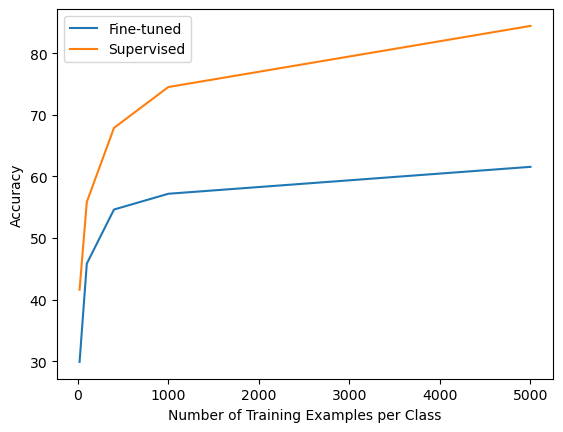
\includegraphics{output.png}}
    \caption{supervised training/fine-tuning on a subset of CIFAR10}
    \label{fig:comparison}
  %\end{center}
  \vspace{0.1\baselineskip}
\end{figure}

\subsection{Train more advanced model}
	由於先前都是使用 ResNet18 去做旋轉的預訓練再對最後幾層或整個網路架構進行調整,自然地我嘗試了 ResNet50 以及 ResNet101,但不論是在旋轉的預測上或是之後應用到圖片的分類上,這兩者的表現都沒有 ResNet18 好,我猜測的原因可能是CIFAR10的資料量還不夠多,因此訓練時,大模型的優勢還沒有顯現出來。因此,最後我採用 DenseNet121 作為我旋轉預測的預訓練以及最後用來作為圖片分類, DenseNet 的網路架構比 ResNet 的更密集,在旋轉預測的預訓練的準確度達到了78.78\%,與使用 ResNet18 的結果差不多,最後經過 fine-tuning 應用到圖片分類時, 準確率達到了 84.85\%,比前面模型提高了 0.74\%。 Table\ \ref{table:comparison3} 呈現了使用 DenseNet121 與 ResNet18 的旋轉預測以及圖片分類的準確度 (accuracy; acc) 比較。 
	
\begin{table}[htb]
	\centering	
	\normalsize
    \newcommand{\z}{\phantom{0}}
    \caption{Simulation results of each model}
    \vspace{0.15\baselineskip}
    %\resizebox{0.5\textwidth}{!}{
	\begin{tabularx}{0.8\textwidth}{@{}lrr@{}}\toprule
		\textbf{Model} & \textbf{rotation prediction acc} & \textbf{classification acc} \\
		\hline
		ResNet18      & 0.7899 & 0.8411 \\ 
		DenseNet121   & 0.7878 & 0.8485 \\
    		\hline
	\end{tabularx}
	%}
	\label{table:comparison3}
   \vspace{0.15\baselineskip}
\end{table}


\subsection{Using ImageNette to train a rotation prediction model}

	此部分我寫了一個 class ImageNetteRotation 去產生 ImageNette 的旋轉資料集,先在 ImageNette 的資料集上做旋轉預測的預訓練接著再應用到 CIFAR10 的圖片分類中,使用的模型為 ResNet18,優化器為 AdamW。 旋轉訓練結束後在 ImageNette 的驗證集上有59.72\% 的準確度,而之後應用到 CIFAR10 的圖片分類任務中,訓練結束後達到了81.97\%,由此可見,即便旋轉預測的預訓練不是在 CIFAR10 資料集上的最後也可以經由調整進而在CIFAR10的圖片分類任務中達到較好的結果。





\bibliographystyle{IEEEtran} 
\bibliography{reference}

\end{document}